\documentclass[Lau, oneside, noexaminfo]{sapthesis}
\usepackage[utf8]{inputenx}
\usepackage{indentfirst}
\usepackage{microtype}
\usepackage[italian]{babel}
%\usepackage{chemformula}
%\usepackage{setspace}
%\usepackage{yfonts,color}
%\usepackage{siunitx}
%\usepackage{comment}
%\usepackage{multirow}
%\usepackage{varioref}
%\usepackage[bottom]{footmisc}
%\usepackage{wrapfig}
%\usepackage{float}
%\usepackage{type1cm}
\usepackage{lettrine}
\linespread{0.9}
%\usepackage{chngcntr}
\usepackage[nottoc, notlof, notlot]{tocbibind}
%\onehalfspacing
%\counterwithout{footnote}{chapter}
\usepackage{hyperref}

\hypersetup{
	%hyperfootnotes=true,			
	%bookmarks=true,			
	colorlinks=true,
	linkcolor=black,
	linktoc=page,
	anchorcolor=black,
	citecolor=black,
	urlcolor=blue,
	pdftitle={Recupero dati da SQLite per attività forensi},
	pdfauthor={Simone Ruberto},
	pdfkeywords={relazione di tirocinio, tesina, tirocinio interno, sapienza, roma, informatica, università}
}

\title{Recupero dati da SQLite per attività forensi}
\author{Simone Ruberto}
\IDnumber{1845772}
\course[]{Informatica}

\courseorganizer{Facolt\`a di Ingegneria dell'informazione, informatica e statistica}
\submitdate{2021/2022}
\copyyear{2022}
\advisor{Prof. Angelo Spognardi}
\advisor{Prof. Marco Cianfriglia}
\coadvisor{Prof. Massimo Bernaschi}
\authoremail{ruberto.1845772@studenti.uniroma1.it}



%we refer to http://ctan.mirrorcatalogs.com/macros/latex/contrib/sapthesis/sapthesis-doc.pdf for an exhaustive description of the sapthesis documentclass.

\newcommand{\SubItem}[1]{
	{\setlength\itemindent{15pt} \item[-] #1}
}

\begin{document}
	
	
	\frontmatter
	\maketitle
	
	\begin{abstract}
		L’oggetto di questo tirocinio è lo studio del funzionamento della tecnologia \textbf{SQLite}, allo scopo di comprendere le caratteristiche tecniche, la struttura dei file SQLite e la gestione dei dati.
		Essendo uno dei motori di database SQL più diffusi al mondo, questa tecnologia è ampiamente utilizzata nelle applicazioni di messaggistica istantanea e in molti programmi, come i web browsers.
		
		\medskip 
		
		Le informazioni contenute in database di questo tipo, spesso, durante investigazioni di tipo forense, sono ritenute di gran valore.
		A questo scopo sono stati sviluppati molti software gratuiti che consentono la visualizzazione dei record attivi, mentre, per quanto riguarda i record eliminati, la maggior parte dei software che ne tentano il recupero sono a pagamento. Alternativamente, il processo di recupero dei record rimossi può essere effettuato a mano.
		
		\medskip
		
		La relazione è divisa in 4 sezioni principali: l’importanza di SQLite nell’\textbf{informatica forense} e una breve introduzione ad essa; il \textbf{formato dei file} di tipo SQLite; il processo di \textbf{eliminazione dei dati} e come contrastarne il recupero e l’implementazione e il funzionamento di \textbf{SQLite Recovery}, uno strumento che automatizza il recupero dei record rimossi.
	\end{abstract}

	
	\newpage\null\thispagestyle{empty}\newpage

	\tableofcontents
	
	\newpage\null\thispagestyle{empty}\newpage
	
	\mainmatter
	
	% !TeX root = ../relazione.tex

\chapter{L’importanza di SQLite nell’informatica forense}


\section{Il motore di database più utilizzato al mondo}
SQLite è presente su un grandissimo numero di dispositivi e i suoi utilizzi possono variare dal conservare le informazioni delle applicazioni di messaggistica istantanea, al conservare i formati dei file utilizzati dalle applicazioni come ad esempio Photoshop Lightroom.

È supportato dalla maggior parte dei dispositivi presenti sul mercato e da quasi tutti i sistemi operativi, anche da quelli integrati. Il numero di smartphone che ne fa un uso attivo ammonta a \textbf{circa 4 miliardi}\footnote{Fonte: SQLite.org; \url{https://www.sqlite.org/mostdeployed.html}} e si stima che ci siano più di un bilione di database SQLite in uso.

La maggior parte delle applicazioni presenti su i nostri smartphone usano database SQLite, per citarne alcune delle più famose: WhatsApp Messenger, Dropbox, Firefox, Safari e Google Chrome.
 	

\section{Quanto è importante recuperare i dati?}
I browser precedentemente nominati utilizzano database SQLite della versione 3 per gestire i dati dell’utente come la cronologia, i cookie e i file scaricati, mentre l’applicazione di messaggistica istantanea WhatsApp lo utilizza per salvare le informazioni su i media scambiati, il registro delle chiamate, i contatti frequenti, i messaggi scambiati e molte altre informazioni, come le informazioni sul dispositivo utilizzato.
Inoltre, anche molte delle applicazioni preinstallate usate dagli smartphone lo usano, come ad esempio l’applicazione per la gestione dei messaggi.

\medskip

I dati detenuti nei database possono in molti casi essere di gran valore durante un’indagine forense.
Se ad esempio un sospettato di un’indagine dovesse \textbf{eliminare} la lista della chiamate, la cronologia di una chat o della navigazione internet, essendo questi dati memorizzati quasi sempre in database di tipo SQLite, potrebbero essere recuperati manualmente o con l’ausilio di software in grado di effettuarne il recupero autonomamente.
I dati acquisiti potrebbero fornire prove schiaccianti nei confronti del sospettato. Infatti, non è raro sentire notizie di persone che tramite chat compromettenti, scambi di contenuti multimediali o ricerche su internet sono stati incriminati.

	
	% !TeX root = ../relazione.tex

\chapter{Introduzione a SQLite}


\section{Cos’è SQLite?}
SQLite è una libreria software scritta nel linguaggio di programmazione C \cite{clanguage}, che implementa un \textbf{motore di database SQL}, ideata da D. Richard Hipp, ma attualmente gestita da un team di sviluppatori.

Il progetto SQLite è iniziato il 29/05/2000 e il team ha come obiettivo di supportarne lo sviluppo fino al 2050\footnote{Dati provenienti dal sito di SQLite: \url{https://www.sqlite.org/}}.
La documentazione e il codice di SQLite sono di dominio pubblico, il codice di SQLite non è Open-Contribution. 

\begin{figure}[ht]
	\centering
	\caption{Logo di SQLite}
	\label{fig:sqlitelogo}
	
\includegraphics[scale=0.5]{assets/logo_sqlite}
\end{figure}

\section{Caratteristiche principali}
L’implementazione del motore del database è;
\begin{itemize}
	\item \textbf{Self-contained}: ha bisogno di pochissime dipendenze per funzionare, infatti, non richiede l’utilizzo di librerie esterne del linguaggio C, ma si limita a utilizzare le routines della libreria standard \cite{cstandardlibrary}
	\item \textbf{Serverless}: il processo che vuole accedere al database scrive e legge direttamente dal file del database sul disco, a differenza di molti altri motori di database SQL, nei quali c’è la necessità di utilizzare un processo ad-hoc
	\item \textbf{Zero-configuration}: SQLite non richiede di essere installato prima dell’utilizzo
	\item \textbf{Transactional}: le transazioni soddisfano le proprietà ACID (Atomicità, Consistenza, Isolamento e Durabilità) \cite{acid}
\end{itemize}
Nonostante il nome possa ingannare SQLite implementa tutte le funzioni di SQL, il “Lite” presente nel nome si riferisce alla ridotta grandezza del file.

SQLite viene testato molto attentamente prima di ogni rilascio ed è molto affidabile, in quanto è utilizzato da miliardi di dispositivi di tutti i tipi senza problemi da ormai quasi due decenni. 

Prima di ogni nuovo rilascio, SQLite viene testato tramite una suite di test automatizzata che esegue milioni e milioni di casi di test che coinvolgono centinaia di milioni di istruzioni SQL, al fine di provare tutti i casi di fallimento.
SQLite ha un’ alta tolleranza ai fallimenti di allocazione della memoria e agli errori di I/O del disco. Le transazioni sono ACID, infatti, anche se interrotte da crash di sistema o interruzioni di corrente, il database rimane in uno stato consistente.
Nonostante tutti i test, anche SQLite presenta dei bug, ma a differenza di altre tecnologie simili il team di sviluppo si impegna a fornire elenchi di bug noti e un changelog sulle modifiche del codice aggiornato al minuto.

\section{Confronto con i motori SQL dotati di server}
Si potrebbe pensare di poter paragonare SQLite ai DBMS \cite{dbms} dotati di server, ma sarebbe sbagliato, in quanto sono concepiti con due scopi differenti. SQLite non compete con MySQL, PostgreSQL o software simili. SQLite nasce con lo scopo di permettere a un programma di poter operare con un database senza dover essere costretto a installare un DBMS o di dover disporre di grandi capacità di memoria.

\medskip
SQLite non è adatto nelle seguenti situazioni;
\begin{itemize}

\item Se si deve permettere l'accesso alla base di dati tramite la rete internet
\item Se è necessario garantire un alto grado di concorrenza, ovvero, se dovessero essere eseguite in uno stesso istante differenti query
\item Se è richiesto un elevato utilizzo della memoria.
\end{itemize}

SQLite è particolarmente indicato nei casi in cui l'archiviazione dei dati avviene localmente nel dispositivo, la quantità dei dati non supera un terabyte di contenuto e non vengono effettuate molte operazioni nello stesso istante. 

SQLite è veloce e affidabile, non richiede configurazioni particolari o attività di manutenzione. 
	
	% !TeX root = ../relazione.tex

\chapter{Il formato dei database file}

A differenza di molti altri motori di database SQL, un database SQLite memorizza tutto all’interno di un singolo file chiamato \textbf{main database file}. 

Il formato dei file SQLite è stabile, retrocompatibile con le versioni precedenti e multipiattaforma, infatti, è possibile copiare lo stesso file su sistemi a 32 e 64 bit o su architetture in cui l’ordine dei byte è di tipo big-endian o little-endian.

I file dei database SQLite sono raccomandati dall’US Library of Congress \cite{uslibraryofcongress}, in quanto il formato massimizza la sopravvivenza e l’accessibilità dei contenuti digitali.

\section{I file Hot Journals}
Con il termine Hot Journals si intendono quei file che contengono le informazioni necessarie per poter ripristinare il database ad uno stato consistente.
SQLite utilizza un secondo file chiamato “rollback journal” o, se l’opzione WAL è disponibile, un file chiamato “Write-Ahead Log”.
In questi file verranno conservate informazioni aggiuntive relative alle transazioni eseguite, che in caso di interruzione del sistema, prima del completamento di una transazione, consentiranno di ripristinare il database ad uno stato consistente eseguendo il rollback di tutte le operazioni eseguite fino al commit precedente.


\section{Pagine}
Un file SQLite è suddiviso in pagine della stessa dimensione. La dimensione in byte di una pagina è compresa da un minimo di 512 byte a un massimo di 65536 byte. 

Ciascuna pagina ha una propria intestazione, la quale permette di ottenere diverse informazioni sulla pagina in cui è situata. 

Il numero massimo di pagine ammonta a ($2^{32}$ – 2), le pagine sono numerate a partire da uno e ciascuna pagina può essere di un determinato tipo a seconda della funzione ricoperta.

\newpage

\section{Header del database}
L’header di un database SQLite consente di determinare le informazioni essenziali per poter operare su questi tipi di file. È collocata nei primi 100 byte del main file e consiste di 32 campi. Le informazioni sono immagazzinate seguendo l’ordine dei byte big-endian.

\medskip
Ad esempio, all’offset 0 leggendo 16 byte si potrà trovare il “Magic Header”, che altro non è che una stringa che identifica che il file è di tipo SQLite.

\medskip

Di seguito è presente una tabella che riassume i campi presenti nell’header:
\begin{figure}[ht]
	\centering
	\caption{Il formato dell'header del database}
	\label{fig:sqlitedatabaseheader}
	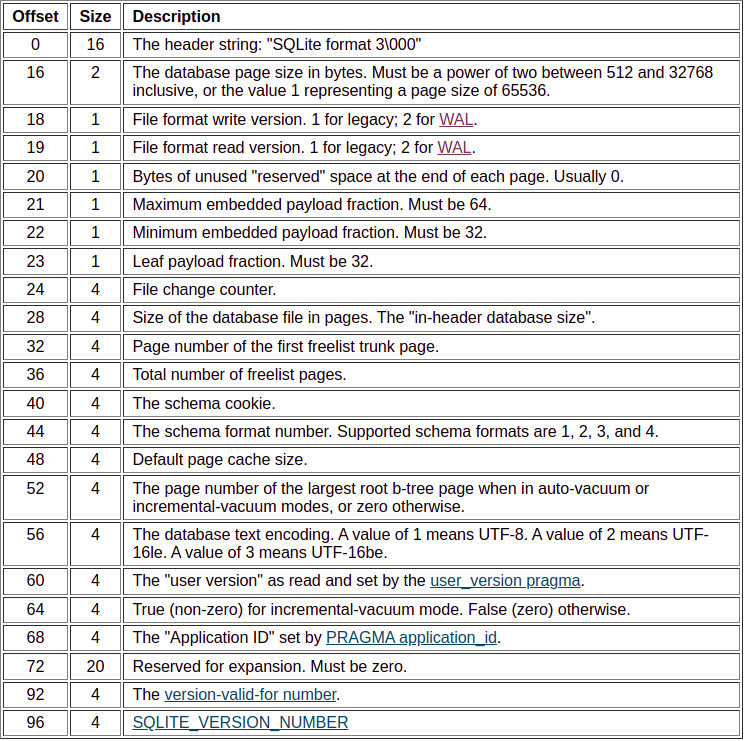
\includegraphics[scale=0.5]{assets/database_header_sqlite}
\end{figure}

\newpage

\section{Freelist}

In ogni istante di tempo un database SQLite potrà avere un certo numero di pagine attive e di pagine non attive. Quelle attive conterranno dei dati validi per il database, mentre, le pagine non attive conterranno dati che non sono più ritenuti validi per la base di dati.
Una pagina diventerà inattiva, quando arriverà a contenere solo informazioni non più valide. 

Le pagine non utilizzate (inattive) verranno memorizzate in delle freelist, che consentiranno di poterle riutilizzare non appena ci saranno ulteriori informazioni da memorizzare.

La freelist è una struttura dinamica organizzata come una lista concatenata, ciascun elemento ha una dimensione di 4 byte seguenti l’ordine dei byte big-endian. Ogni elemento della lista consiste di due interi da 2 byte ciascuno, il primo intero è il numero della seguente pagina non attiva nella freelist, mentre, il secondo intero è il numero di inserimenti all’interno di quella pagina. Per segnalare il termine degli elementi nella freelist, SQLite memorizzerà nell’ultimo elemento della lista il valore 0 per identificarne il termine.
All’interno dell’header del database sono presenti delle informazioni utili per operare con le freelist;
\begin{itemize}
\item All'offset 36 è presente un intero di 4 byte, che rappresenta il numero delle pagine nella freelist
\item All’offset 32 è presente il numero della prima pagina all’interno della freelist
\end{itemize}


\section{Le pagine di tipo b-tree}

SQLite utilizza come algoritmo per memorizzare le informazioni il b-tree. Questo algoritmo ci consente di memorizzare le informazioni come coppie di chiave:valori.

\medskip

Ciascuna pagina b-tree è di uno dei seguenti tipi;
\begin{itemize}
\item interna di tipo indice
\item interna di tipo tabella
\item foglia di tipo indice
\item foglia di tipo tabella
\end{itemize}

Le pagine foglie contengono le chiavi e, nel caso in cui la pagina sia di tipo tabella, conterranno anche i dati associati alle chiavi. Mentre, per quanto riguarda le pagine interne, esse conterranno solamente le chiavi e per ogni chiave il puntatore associato alla pagina figlia.

\newpage
	
\subsection{Struttura}

Ogni pagina è suddivisa nelle seguenti sezioni ordinate;

\begin{figure}[ht]
	\centerline{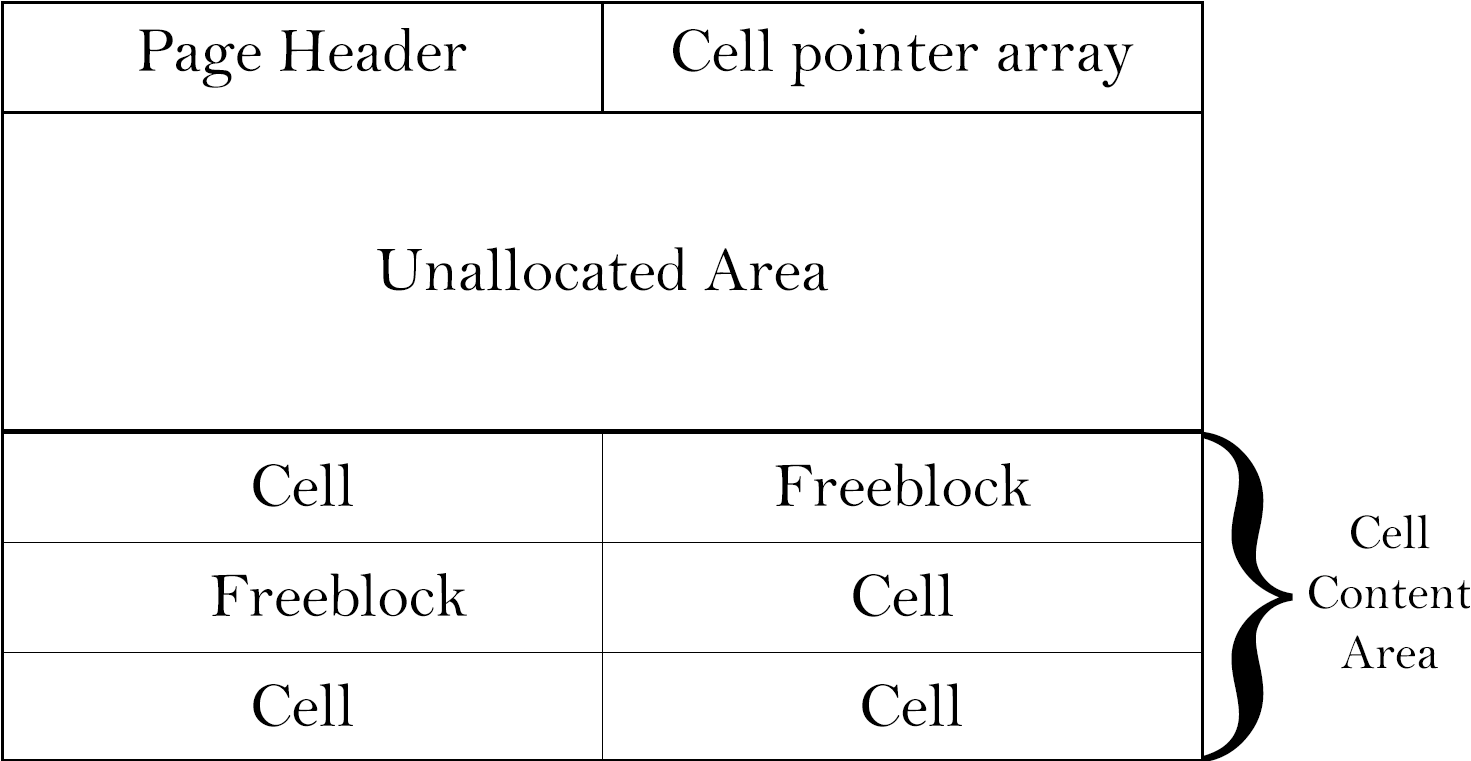
\includegraphics[scale=0.25, ]{assets/b-tree-page-structure}}
	\caption{La struttura di una pagina b-tree}
	\label{fig:btreepagestructure}
	
\end{figure}

\begin{itemize}
\item I primi 100 byte rappresentano l’header del database (ciò vale solo per la prima pagina), questa sezione non è rappresentata nella figura precedente
\item Verranno utilizzati dagli 8 ai 12 byte per rappresentare l’header della pagina
(8 byte per le pagine foglie e 12 per le pagine interne)
\item Un array che contenente i puntatori alle celle
\item L’area contenente lo spazio non allocato presente all’interno della pagina
\item L’area contenente il contenuto delle celle
\item L’area riservata
\end{itemize}

L’array contenente i puntatori alle celle userà un numero di byte pari al numero di celle puntate per 2 byte (ciascun elemento dell’array rappresenterà l’offset al contenuto della cella dall'inizio della pagina).

L’area non allocata contiene dei byte che non sono utilizzati, ma che potranno permettere all’area contenente il contenuto delle celle di espandersi. Quest’area non appena il database sarà costruito verrà inizializzata a 0. 

L’area riservata può essere utilizzata dalle estensioni di SQLite per fornire funzioni aggiuntive, come l’estensione SQLite Encryption Extension (SEE), la quale permette ad un applicazione di scrivere e leggere su database cifrati.

\newpage

\subsection{Il formato dell’header}

Come già detto in precedenza, l’header della pagina potrà occupare 8 o 12 byte, a seconda del tipo.

\medskip

Di seguito ne viene riportata la struttura;

\begin{itemize}
\item Il primo byte dell’header indicherà il tipo di pagina b-tree
\SubItem{Il valore 2 (0x02) indica una pagina interna di tipo indice}
\SubItem{Il valore 5 (0x05) indica una pagina interna di tipo tabella}
\SubItem{Il valore 10 (0x0a) indica una pagina foglia di tipo indice}
\SubItem{Il valore 13 (0x0d) indica una pagina foglia di tipo tabella}

\item I successivi due byte indicano l’inizio del primo freeblock nella pagina, o 0 se quest'ultimo non è presente
\item Il quarto e il quinto byte rappresentano un valore intero indicante il numero di celle nella pagina, con il termine di cella si fa riferimento a un record.
\item Nei successivi due byte troviamo l’offset dall’inizio della pagina all’inizio dell’area contenente le celle.
\item Nel byte successivo è memorizzato il numero dei byte liberi frammentati all’interno dell’area contenente le celle.
\item Nelle pagine interne ci saranno 4 ulteriori byte per conservare il puntatore più a destra che permette di trovare la cella con la chiave più grande.
\end{itemize}

\subsection{Freeblock}
I freeblock sono strutture dati utilizzate da SQLite per identificare lo spazio non utilizzato all'interno dell'area contenente le celle di ciascuna pagina.
Queste aree vengono memorizzate per permettere a SQLite di poterle riutilizzare. 
Come illustrato in precedenza, all'interno dell'header della pagina c'è un campo che sta a indicare l'offset dall'inizio della pagina al primo freeblock.
I freeblock sono organizzati come una catena, infatti, ciascun elemento è composto da 4 byte; i primi due identificano l'offset al prossimo freeblock e i successivi due la grandezza del freeblock in byte.
Se la grandezza del freeblock dovesse essere uguale a 0 allora ciò indicherebbe che non sono presenti ulteriori freeblock nella pagina.

\newpage

%\subsection{Spazio non allocato}
%a

%\subsection{Area contenente le celle}
%a

%\subsection{Area riservata}
%a

\section{Tipi di dati}
Prima di poter illustrare il formato dei record, è necessario spiegare due tipi di dati, che vengono utilizzati da SQLite per codificare le informazioni dei record.

\paragraph{Il tipo di dato varint}
\hfill \break
SQLite fa un ampio uso delle variabili varint (Variabile-Length Integers), esse permettono di rappresentare interi senza segno e hanno una lunghezza che può variare da 1 byte ai 9 byte. Questo tipo di dato gode delle seguenti proprietà;

\begin{itemize}
\item Rappresentare interi piccoli utilizzando meno byte
\item Conoscere la lunghezza in byte della variabile guardando il primo byte
\item Avere l'ordine lessicografico e numerico identico, ciò permette di poter utilizzare queste variabili come chiavi. 
\end{itemize}


\paragraph{I codici serial types}
\hfill \break
Sulla base dei valori rappresentati dalle variabili spiegate in precedenza, all'occorrenza, ovvero nel momento in cui andremo a identificare i campi da cui è composto un record, SQLite utilizza i serial types per codificare il tipo di un campo di un record e la dimensione del contenuto in byte del campo.

\medskip
\medskip
Per conoscere queste informazioni, a seconda del valore intero memorizzato dalla variabile varint, seguiremo le regole riportate nella tabella seguente:

\medskip
\begin{figure}[ht]
	\centerline{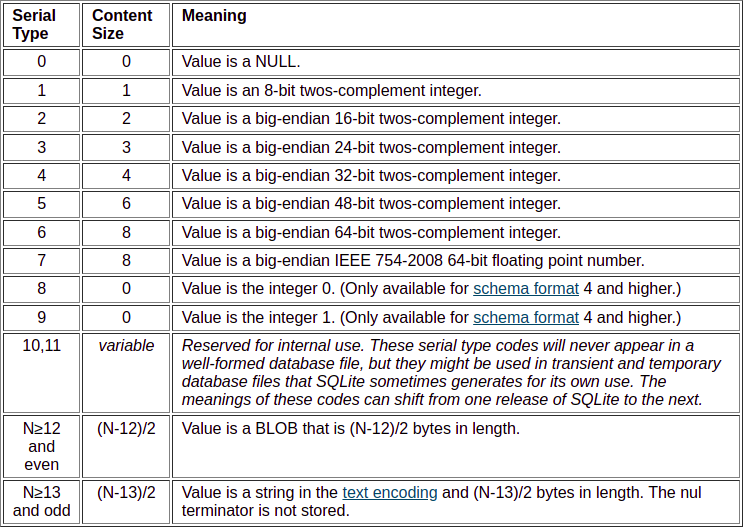
\includegraphics[scale=0.5, ]{assets/serialtypes}}
	\caption{Codici Serial Type}
	\label{fig:serialtypes}
	
\end{figure}

\section{Il formato dei record}
All'interno dell'area contenente i record di ciascuna pagina sono presenti un numero arbitrario di byte utilizzati per memorizzare i record.
\medskip

Ciascun record segue questo formato:
\begin{figure}[ht]
	\centerline{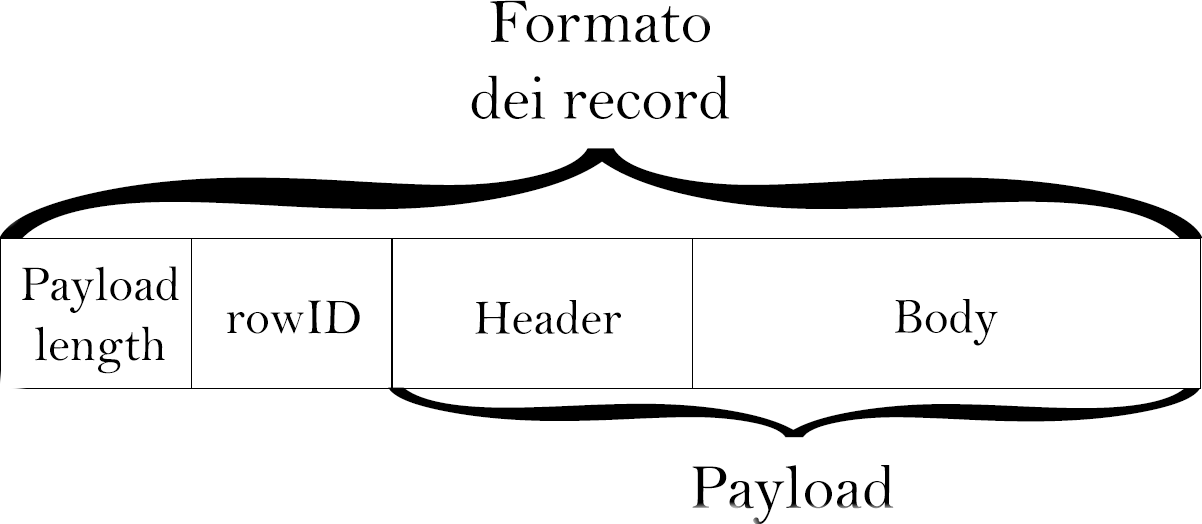
\includegraphics[scale=0.25, ]{assets/record_format}}
	\label{fig:recordformat}
\end{figure}

Per rappresentare questo formato si fa un grande uso delle variabili di tipo varint. 

Il primo campo Payload length, infatti, è rappresentato da una variabile varint che sta a indicare il numero di byte che costituiscono il payload. È presente una seconda variabile varint che memorizza l'id del record. La sezione successiva (payload) memorizza il contenuto delle colonne del record e le informazioni, per risalire al tipo di campo e la lunghezza in byte del contenuto.


\paragraph{Payload}
Questa sezione è a sua volta suddivisa in due sottosezioni: l'header e il body.
Attraverso l'header si è in grado di risalire al numero di campi da cui è composto il record, il tipo di ciascun campo e la dimensione in byte del contenuto.
Queste informazioni sono codificate mediante l'utilizzo del tipo di dato varint e, con l'ausilio dei codici serial types, si riusciranno a identificare i tipi dei campi e la dimensione in byte.
\medskip

Di seguito è presente un'immagine che illustra la struttura dell'header;


\begin{figure}[ht]
	\centerline{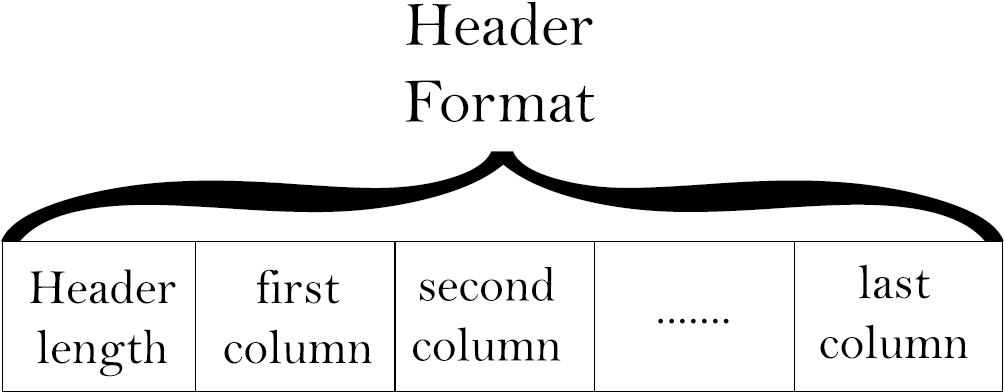
\includegraphics[scale=0.25, ]{assets/record_header_format}}
	\label{fig:recordheaderformat}
\end{figure}

Terminata l'header troviamo il body, all'interno del quale sono presenti diversi byte che ci permettono, sulla base delle informazioni ottenute tramite l'header, di risalire al contenuto del record e quindi dei singoli campi che lo compongono.

\newpage

\paragraph{Esempio}
Per comprendere meglio ciò che è stato precedentemente illustrato, viene presentato un esempio, che, a partire da una sequenza di valori esadecimali rappresentanti un record, ne ricostruisce il contenuto. Questi valori sono stati ottenuti da una pagina foglia di tipo tabella, più precisamente dall'area non allocata.
\medskip

La sequenza di valori presa in esempio è la seguente:

\begin{figure}[ht]
	\centering
	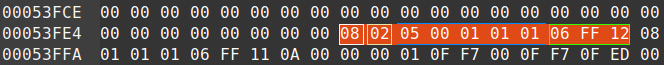
\includegraphics[scale=0.6, ]{assets/hex_record}
	\label{fig:hexrecord}
\end{figure}

Ciascuna sezione che va a comporre il record è contraddistinta da un colore differente.


Ad esclusione dei valori presenti nel body del payload, i restanti sono codificati come variabili di tipo varint. 
Per come viene decodificato questo tipo di dato, i valori minori di 241 vengono convertiti in valori interi come una semplice conversione da esadecimale a intero, per ulteriori informazioni sull'algoritmo utilizzato per codificare e decodificare le variabili varint \cite{varint}.


\begin{itemize}
\item Il primo valore (08) rappresenta il payload length e indica che il payload è composto da 8 byte.
\item Il successivo valore (02) indica che l'id del record è 2. 
\item L'header del payload inizia con il valore 5, che sta a indicare la lughezza in byte dell'header
\item Successivamente troveremo tante variabili varint quante sono le celle che vanno a comporre il record, per ogni variabile varint useremo i codici serial types per ricavarne il tipo e la lunghezza in byte;
\SubItem{Il valore 0 non ci dà informazioni sul tipo della cella, nè della sua lunghezza in byte. Indica solamente che c'è un campo (la row id, di cui abbiamo già il contenuto)}.
\SubItem{Il valore 1 sta a indicare che il contenuto della seconda cella è un numero intero di 8 bit complemento a 2.}
\SubItem{Lo stesso vale per i successivi due valori esadecimali (01 01)}
\item Terminata l'header del payload, troviamo il body evidenziato in verde, tramite questo, e sulla base delle informazioni acquisite dalla sezione precedente, siamo in grado di ottenere il contenuto delle celle.
\SubItem{La seconda cella del record è un intero di 8-bit in ca2, quindi di valore 6}
\SubItem{Lo stesso vale per la terza e quarta cella, cioè -1 (FF) e 18 (12)}
\end{itemize}

\newpage

Ottenute queste informazioni siamo in grado di ricostruire la struttura del record e il contenuto. Ovviamente non possiamo affermare nulla sulla tabella di appartenenza. Vedremo in seguito come poter ottenere un insieme di tabelle potenziali sulla base delle informazioni ottenute dall'header.

\medskip

\begin{figure}[ht]
	\centering
	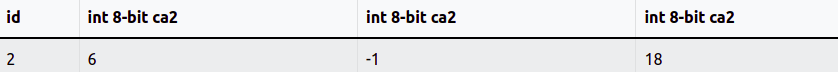
\includegraphics[scale=0.45, ]{assets/record_parse}
	\caption{Record convertito}
	\label{fig:recordparse}
\end{figure}


	
	% !TeX root = ../relazione.tex



\chapter{Risorse utili al recupero dei record cancellati}
Quando viene rimosso un record o quando viene eseguita un'operazione di drop su una tabella, in SQLite almeno che non siano attivate particolari direttive, oppure non sia stato eseguito il comando vacuum, il contenuto rimosso non viene sovrascritto. Seguirà una breve panoramica su tutte le risorse in cui potrebbero essere presenti i dati rimossi.

\section{Le freelist}
Come già detto in precedenza, un database SQLite potrebbe avere zero o più pagine che non sono in uso attivo. 

Queste pagine vengono rese inattive non appena il contenuto memorizzato al loro interno viene rimosso dal database, ad esempio quando viene eseguito il drop su un'intera tabella.

Le pagine inattive potrebbero contenere vecchi record rimossi o intere tabelle rimosse.

Nella sezione 3.4 è stata illustrata la struttura delle freelist, vedremo adesso più nel concreto come reperire le aree di memoria di queste pagine.

Una volta appurato che ci siano pagine inattive e ottenuto il numero della prima pagina attraverso l'header del database, con questa semplice equazione possiamo calcolare l'offset dall'inizio del file all'inizio della pagina.

\medskip

Indirizzo della prima pagina nella freelist:

\medskip

\mbox{(4 byte (BE) all’offset 32 dell’inizio del file – 1) * grandezza in byte di una pagina}

\medskip

Essendo una pagina b-tree, questa presenterà un header come illustrato in precedenza, che ci fornirà le relative informazioni della pagina come il tipo, il numero di record e se ci sono freeblock.

Per ottenere tutti gli indirizzi di tutte le pagine, itereremo questa procedura per tutti gli elementi che vanno a comporre la freelist. Ogni pagina ottenuta potrebbe contenere record rimossi nella sezione contenente i record, nei freeblock e nell'area non allocata. 

\section{I freeblock e l'area non allocata}

A differenza della sezione contenete i record di una pagina, nei freeblock e nelle aree non allocate potrebbero essere presenti anche i frammenti di record. La procedura di recupero potrebbe generare molti falsi record, ma se un database non dovesse presentare pagine inattive, l'unico modo per cercare di recuperare i record rimossi è ricorrere a queste aree.

\medskip

I freeblock sono aree di memoria non utilizzate presenti all'interno delle pagine nella sezione contenete i record. Se il numero di byte di queste aree dovesse risultare maggiore di una certa soglia stabilita da SQLite, significherebbe che la sezione è molto frammentata, SQLite per deframmentare quest'area, sposterebbe il contenuto dei freeblock nell'area non allocata e rimuoverebbe i freeblock.


	
	
\chapter{Contrastare il recupero dei dati}
SQLite per evitare che i dati rimossi possano essere recuperati, mette a disposizione una serie di direttive e di comandi che permettono in diverse modalità la sovrascrittura dei dati rimossi. Queste direttive di default sono disattivate. 
 	
\section{Le direttive}
\paragraph{auto vacuum}
Quando non è attiva, all'eliminazione dei dati dal database, la grandezza del file principale rimane invariata, le pagine inattive verranno aggiunte alla freelist e riutilizzate all'occorrenza.
Questa direttiva può operare in 3 modalità;

\begin{itemize}
\item 0 è lo stato di default, ovvero la direttiva risulta essere disattivata
\item 1 le pagine inattive verranno spostate alla fine del file e la dimensione verrà troncata ad ogni commit di una transazione
\item 2 a differenza dello stato precedente, l'operazione descritta avverrà ad ogni invocazione della direttiva incremental vacuum
\end{itemize}


Bisogna notare che questa direttiva non evita la frammentazione dell'area contenente le celle nelle pagine (i freeblock).

\paragraph{secure delete}
Quando abilitata, questa direttiva, all'occorrenza dell'eliminazione dei dati provvederà a sovrascrivere il contenuto con degli 0. Questa operazione ha un forte impatto sulle performance, ma consente di non lasciare tracce quando un contenuto viene rimosso o modificato.

Oltre ad essere abilitata supporta un ulteriore modalità chiamata fast, la quale consiste in una via di mezzo tra essere abilitata e disabilitata. Più nello specifico fa sì che venga sovrascritto il contenuto se e solo se non aumenta la quantità di operazioni di input/output, a discapitato di un maggior numero di cicli della CPU. In questa modalità verranno lasciate delle tracce nella pagine presenti nella freelist.

\section{Il comando vacuum}
Questo comando permette la ricostruzione del database nello spazio minimo richiesto. All'esecuzione verranno rimosse le pagine inattive presenti nella freelist, verranno rimossi i freeblock dall'interno dell'area contenente le celle delle pagine e verranno sovrascritte tutte quelle aree marcate come eliminate disponibili per il riuso.


	
	% !TeX root = ../relazione.tex

\chapter{SQLite Recovery}
SQLite Recovery è uno script scritto in python nella versione 3.8.10.  

Quest'ultimo permette di recuperare i record cancellati, più nello specifico utilizza lo spazio non allocato delle pagine foglie b-tree di tipo tabelle e dei freeblock presenti nelle pagine di questo tipo.

Lo script è stato testato su file SQLite del formato 3.

Lo strumento opera in due modalità che saranno eseguite entrambe ad ogni esecuzione.

La prima modalità si limiterà a prendere i dati delle aree in cui potrebbero essere presenti dei record e li immagazzinerà in un file chiamato raw\string_data.tsv.

La seconda modalità, a partire dai dati ottenuti dalla modalità precedente, cercherà di parsare i record o frammenti di record.

Terminata l’esecuzione sarà possibile visualizzare i record ottenuti tramite il file “report.html” (assicurarsi che il browser utilizzato per l’apertura del file html permetta il caricamento di file json locali), per maggiori informazioni visitare la pagina GitHub \footnote{GitHub repository: \url{https://github.com/Er-Simon/Sqlite3-restore-deleted-records}}.


\section{Ambiente di testing}
Per testare il corretto funzionamento dello script, è stato realizzato attraverso l'ausilio dell'applicazione di messaggistica istantanea Whatsapp un ambiente di testing. Innanzitutto, è stato creato un account attraverso il quale è stata simulata una conversazione con un altro account. Durante questa conversazione c'è stato uno scambio di un totale di 11 messaggi, dei quali 4 di tipo testo, 3 immagini di cui una con la descrizione, 2 messaggi vocali e 2 contatti.

Successivamente sono stati rimossi diversi messaggi: una delle 3 immagini scambiate, un contatto e un messaggio vocale.

Prima della rimozione è stato esportato il file SQLite generato dall'applicazione di Whatsapp ed è stato eseguito il comando vacuum per vedere se ricostruendo il database fosse cambiata la dimensione, in modo da capire se ci fossero già eventuali tracce (come i freeblock, i dati nelle aree non allocate o delle pagine inattive). Eseguito il comando, la dimensione è rimasta invariata.

È stato eseguito nuovamente il comando dopo l'eliminazione e si è notato che il file ottenuto era di diversa dimensione. Raggiunto questo risultato si è compreso che qualche messaggio eliminato dovesse essere ancora presente all'interno del file, ma contrassegnato come rimosso.

\section{Patterns}
Precedentemente è stata illustrata la procedura di recupero dei record. Come si è notato, il recupero ha permesso di ottenere le informazioni su i tipi di dati contenuti nelle celle e il contenuto di quest'ultime.
Sulla base delle informazioni ottenute dall'intestazione del record (ovvero i tipi dei campi) e presupponendo che queste informazioni siano corrette, verrà illustrato il procedimento per costruire per ogni record un insieme di tabelle candidate di appartenenza. 
Prima di tutto lo script analizzerà lo schema del database per ricavare per ogni tabella un pattern sul tipo di dati delle celle. Per ogni tabella verrà quindi preso il nome, il numero di campi da cui è costituita e per ogni campo verrà preso il nome e i suoi flag, cioè se primary key, se not null e il tipo di dato.
Ottenute queste informazioni, si è in grado di costruire un insieme di tabelle candidate per ogni record trovato, basandosi sul confronto cella per cella con le informazioni ottenute dallo schema.
Una ricerca di questo tipo potrebbe produrre anche falsi risultati: si potrebbe pensare di includere come criterio di ricerca anche l'id del record e confrontarlo con gli id delle righe non eliminate presenti all'interno del database.

\section{Risultati ottenuti}
Eseguito lo script adottando il criterio di ricerca precedentemente illustrato si è arrivati a un numero cospicuo di record e di tabelle candidate, bisogna però considerare che il database di Whatsapp è costituito da 36 tabelle molte delle quali con lo stesso schema.

Molti dei record trovati sono falsi positivi, in quanto, l'intestazione del record eliminato non risultava essere intatta. Tra i record trovati però ci sono anche i record relativi ai messaggi eliminati.
Più nello specifico si sono recuperati i record rappresentanti l'invio del contatto Whatsapp, in cui sono presenti le informazioni relative a quando è avvenuto il messaggio, il mittente, il destinatario e le informazioni sul contatto (nome, numero di cellulare, ecc..).
Whatsapp solo per questo messaggio ha generato 4 record in 4 differenti tabelle.
Il record rimosso contente queste informazioni è stato recuperato all'interno dell'area non allocata di una pagina.
Inoltre, sono stati recuperati anche i record generati a seguito dell'invio dell'immagine e le relative informazioni, come il path in cui è situtata all'interno del dispositivo, quando è stato inviato il messaggio, il mittente e il destinatario, la thumbnail dell'immagine, la grandezza in byte e molte altre informazioni.
I record relativi all'immagine sono stati trovati sia nelle aree non allocate che nei freeblock.
Mentre, per quanto riguarda il messaggio vocale, lo script non è stato in grado di recuperare alcun record.

Per avere un ulteriore riscontro sul corretto recupero dei record, dono stati confrontati i risultati ottenuti con un altro software chiamato FQLite \cite{fqlite}.
Visionando i risultati ottenuti da entrambi i software, si è notato che FQLite, a differenza dello script SQLite Recovery, ha trovato meno record falsi positivi, ma, per quanto riguarda i record validi, sono stati trovati gli stessi record da entrambi.
Questo dovrebbe essere dovuto al fatto che FQLite nel criterio di ricerca include anche il confronto della chiave primaria della riga trovata, con le chiavi primarie delle righe presenti nelle tabelle candidate.

\section{Implementazione}
I file riportati di seguito fanno riferimento alla repository GitHub menzionata in precedenza.

\medskip

Il file main.py utilizzerà la variabile database\string_path per contenere il path in cui è collocato il file del database.

\medskip

Verrà creato un oggetto della classe database (database\string_parser.py) rappresentante il file situato al database\string_path, durante la creazione verificherà che il file esista, otterrà la dimensione in byte del file e verrà controllato che l’utente abbia i permessi di lettura. 
Se le condizioni precedenti sono verificate procederà ad aprire il file in modalità “rb” (reading binary) e ne leggera i primi 100 byte (l’header del database).
Tramite l’header controllerà che i primi 16 byte convertiti in hex corrispondano alla stringa “53514c69746520666f726d6174203300”, in quanto ogni SQLite database file valido inizia con i precedenti byte.
Leggerà i successivi 2 byte (offset 16) per acquisire la grandezza delle pagine in byte e successivamente all’offset 56 ne leggerà ulteriori 4 per ottenere un intero rappresentante la codifica utilizzata per immagazzinare le stringhe nel database.

\medskip

Terminata la fase di inizializzazione verrà creato un oggetto della classe report presente nel file (report\string_builder.py). Questo oggetto rappresenta le informazioni ottenute durante l’esecuzione dello script, inoltre, al termine dell’esecuzione genererà un file “report.html” per visualizzare le informazioni ottenute.

\medskip

Aperto il flusso di dati del file e ottenute le informazioni essenziali per operare avrà luogo la prima modalita;

\medskip

Verrà aperto in scrittura il file raw\string_data.tsv in cui saranno scritte le informazioni raccolte.
Verrà letto il file specificato da database\string_path fino alla fine andando ad incrementare l’offset ad ogni lettura di un numero di byte pari alla grandezza di una pagina, così facendo ogni volta andremo a lavorare su una diversa pagina alla volta.

\medskip

Per ogni pagina verranno acquisite innanzitutto le informazioni dall’header.
Verrà letto il primo byte per capire il tipo di pagina e quindi la tipologia di dati contenuti all’interno. 
Se il byte convertito in int vale 13 allora la pagina in questione è foglia di tipo (tabella) ovvero dove sono contenuti i dati (record).

\medskip

Successivamente verranno letti i seguenti due byte per capire a quanto ammonta l’offset al primo freeblock (i freeblock sono strutture utilizzate da SQLite per identificare lo spazio non allocato in una pagina).

I due byte seguenti rappresentano il numero di celle nella pagina, questa informazione ci occorrerà per calcolare il numero di byte occupati dal cell pointer array che è situato dopo l’header.

\medskip


Nei due byte successivi troviamo l’offset all’inizio dell’area della pagina contenente le celle e al byte seguente il numero di byte liberi frammentati contenuti all’interno dell’area in cui sono le celle.

\medskip


Ottenute queste informazioni possiamo calcolare la grandezza dell’area non allocata e l’offset dall’inizio della pagina all’inizio dell’area non allocata.

\medskip

Inizio dell’area non allocata:

\medskip

offset inizio pagina + 8 byte header + (2 byte * numero di celle nella pagina)

\medskip

Lunghezza dell’area non allocata:

\medskip

offset all’inizio dell’area della pagina contenente le celle -  8 byte header - (2 byte * numero di celle nella pagina)

\medskip


Verrà letto il contenuto dell’area non allocata è memorizzato all’interno del file raw\string_data.tsv.
Prima di essere scritto sul file il contenuto verrà ripulito dei byte non printabili.

\medskip

Come già accennato prima sqlite utilizza i freeblock per identificare lo spazio non allocato sparso all’interno della pagina, i freeblock sono organizzati come una catena di blocchi.

\medskip

Dall’header della pagina abbiamo letto l’offset al primo freeblock, se il valore è diverso da 0 allora ci sposteremo all’offset indicato + l’offset dall’inizio del file alla pagina corrente.

\medskip

Nei primi due byte è indicato l’offset al prossimo freeblock o 0 se non presente, nei successivi due byte la grandezza del freeblock attuale (inclusi i 4 byte letti).

\medskip

Leggeremo il contenuto del freeblock e lo immagazzineremo nel file rimuovendone i caratteri non printabili.

\medskip

Eseguiremo questi passaggi fino a quando l’offset al prossimo freeblock non sia pari a 0.

\medskip

Terminata la modalità uno i dati delle aree non allocate verranno passate come input alla seconda modalità.

\medskip

Prima di aver luogo la seconda modalità ha bisogno di sapere la struttura delle tabelle del database.

\medskip

Tramite la funzione get\string_patterns presente all’interno del file patterns\string_extractor verrà aperto il database tramite il modulo sqlite3.

\medskip

La funzione eseguirà una query sulla tabella sqlite\string_master per ottenere il nome di tutte le tabelle presenti all’interno del database.

\medskip

Per ciascuna tabella ottenuta tramite l’istruzione PRAGMA table\string_info(nome\string_tabella) verranno ottenute le informazioni relative ai campi (nome, tipo\string_di\string_dato, primary\string_key).

\medskip

Le informazioni ottenute verranno immagazzinate all’interno di un dizionario con questa struttura:

\begin{figure}[ht]
	\centering
	\caption{Logo di SQLite}
	\label{fig:sqlitelogo}
	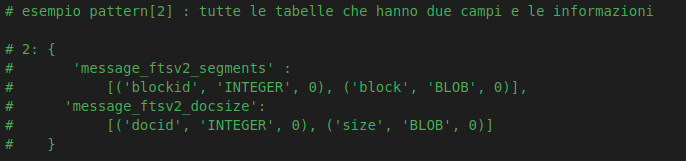
\includegraphics[scale=0.5]{assets/recovery_dict}
\end{figure}

Il dizionario ci consentirà di trovare un insieme di tabelle candidate a seconda della struttura del record trovato.

Il informazioni sullo schema delle varie tabelle varranno inoltre utilizzate dalla classe report.

\newpage

Seconda modalità:

Ogni area non allocata verrà passata alla funzione analyze\string_unallocated\string_area presente all’interno del file record\string_parser.py, la funzione per ogni valore != 0 farà partire la funzione parse\string_varint\string_to\string_record (perché potrebbe essere un possibile record o frammento di record).

La funzione parse\string_varint\string_to\string_record, per aver luogo utilizzerà inoltre l’area in bytes da analizzare convertita in variabili varint (un particolare tipo di dato utilizzato da sqlite per rappresentare numeri interi).

\medskip

Ogni record in SQLite è composto da una variabile varint rappresentante il numero di bytes del payload, una seconda variabile varint rappresentante il row id e da un insieme di byte rappresentante il payload.

Il payload si suddivide in un header e un body, l’header inizia con una variabile varint rappresentante il numero di bytes nell’header, seguita da una o più varint (una per colonna) rappresentanti i serial type che ci indicano il tipo di dato in quella colonna e la size in byte del dato.

\medskip

Terminato l’header inizia il body, tramite i serial type ottenuti precedentemente sapremo riconoscere le colonne nel body e quanti byte sono utilizzati per contenere il valore della relativa colonna.

\medskip

Ottenuto un possibile record proveremo a vedere se ci sono tabelle candidate, ovvero seguenti la medesima struttura. Se la struttura è associata ad almeno ad una tabella, aggiungo il record ottenuto al dizionario della classe report, che ci consentirà successivamente di visualizzarlo tramite una comoda interfaccia. 

\section{Interfaccia}
Dopo aver eseguito lo script, verranno prodotti tre file; un primo file contente i byte presi dalle aree in cui potrebbero essere presenti dei record rimossi, un secondo file json contenente le informazioni sull'esecuzione dello script, su i record trovati e sulle relative tabelle candidate e, infine, un terzo file html che consente la visualizzazione del file json.
Questa interfaccia è stata realizzata mediante l'utilizzo del framework boostrap. Per consentire il caricamento in modo asincrono del file json è stata usata la libreria javascript jQuery. \cite{jquery} Per rendere la pagina interattiva, sono stati gestiti una serie di eventi da parte dell'utente mediante semplici funzioni javascript.
L'interfaccia è stata resa responsive tramite la tecnologia grid-system \cite{boostrapgridsystem} fornita dal framework boostrap, in modo da essere utilizzata sia su dispositivi desktop che mobili.

\begin{figure}[ht]
	\centerline{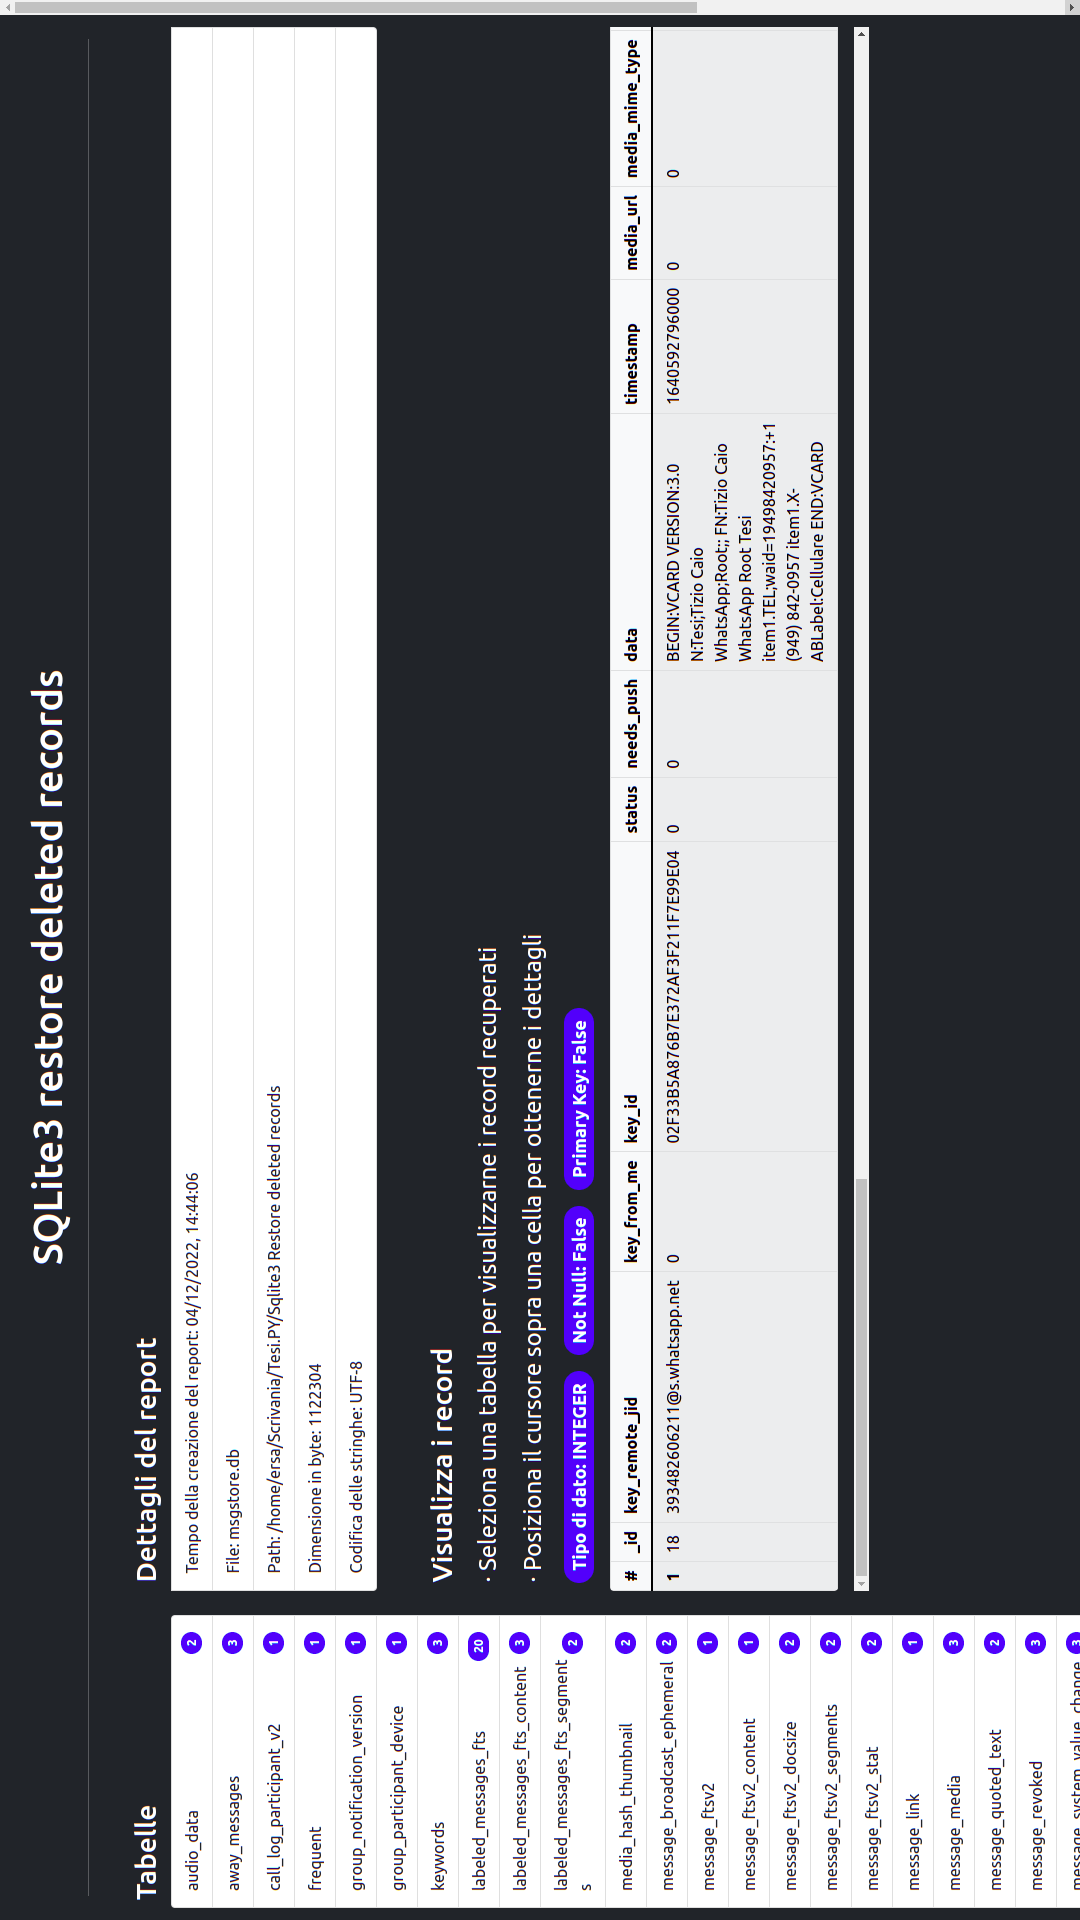
\includegraphics[scale=0.35, ]{assets/interface}}
	\caption{Interfaccia di SQLite Recovery}
	\label{fig:interface}
\end{figure}



	
	% !TeX root = ../relazione.tex

\chapter{Conclusioni}
In questa relazione è stato descritto il lavoro svolto durante l’attività di tirocinio.

È stata illustrata una breve panoramica sulla tecnologia SQLite, sul suo utilizzo e sull'importanza che possono avere i dati contenuti all'interno dei file SQLite.
Sono state riportate le caratteristiche principali alla base di questa tecnologia e si è cercato di fare un confronto con i motori SQL relazionali tradizionali.
Inoltre, sono stati illustrati i componenti principali per comprendere al meglio il formato dei file di tipo SQLite ed è stato mostrato il processo di recupero dei record a partire da valori esadecimali.
Sono state spiegate le risorse utili al recupero dei record, le direttive e i comandi per evitare che i dati possano essere recuperati.
È stato presentato SQLite Recovery, uno script in grado di automatizzare il processo di recupero dei record da file SQLite e i suoi sviluppi futuri. 

\medskip

Durante il tirocinio ho avuto modo di applicare alcuni dei concetti appresi nei
vari corsi di studio. Ho avuto inoltre l’opportunità di approfondire e imparare alcune tecnologie e approcci, migliorando la mia conoscenza ed esperienza di programmazione.
Ho avuto modo di comprendere la tecnologia SQLite, la sua importanza nelle attività forensi e il suo utilizzo su larga scala.



\section{Sviluppi futuri di SQLite Recovery}
SQLite attualmente supporta le seguenti funzioni;

\begin{itemize}
	\item recuperare i record o i frammenti dallo spazio non allocato delle pagine foglie di tipo tabella
	\item recuperare i record dai freeblocks presenti nelle pagine foglie di tipo tabelle
	\item supporta le diverse codifiche utilizzate da SQLite per immagazzinare le stringe (UTF-8, UTF-16BE, UTF-16LE)
	\item salvare i bytes delle aree non allocate e dei freeblocks su un file tsv
	\item visualizzare i dati ottenuti tramite una interfaccia
\end{itemize}	
	
In futuro questo script potrebbe essere ampliato andando a implementare ulteriori funzioni come: dare la possibilità di recuperare i record dalle pagine presenti nella freelist, recuperare i record delle tabelle eliminate, aumentare le informazioni riportate all’interno dell’interfaccia e dare la possibilità di ripristinare i file SQLite corrotti.


	
	\newpage\null\thispagestyle{empty}\newpage

	\backmatter
	\phantomsection
	\begin{thebibliography}{17}
		
		%\bibitem{sqlite:mostdeployed}
		%\textbf{Most Widely Deployed SQL Database Engine}. %\url{https://www.sqlite.org/mostdeployed.html}
		
		\bibitem{clanguage}
			\textbf{C programming language}.
			\url{http://www.open-std.org/jtc1/sc22/wg14/}
			
		\bibitem{cstandardlibrary}
			\textbf{C standard library}. \\
			Wikipedia contributors,
			\url{https://en.wikipedia.org/wiki/C_standard_library}
		
		\bibitem{acid}
			\textbf{ACID (atomicity, consistency, isolation, durability)}. \\
			Wikipedia contributors,
			\url{https://en.wikipedia.org/wiki/ACID}
		
		\bibitem{uslibraryofcongress}
			\textbf{LoC Recommended Storage Format}. (21-08-2020) \\
			\url{https://www.loc.gov/preservation/digital/formats/fdd/fdd000461.shtml#local}

		\bibitem{dbms}
			\textbf{Database management system}. \\
			Wikipedia contributors, \url{https://it.wikipedia.org/wiki/Database_management_system}
			
		\bibitem{varint}
			\textbf{Variable-Length Integers}. \\
			SQLite Developers, 
			\url{https://sqlite.org/src4/doc/trunk/www/varint.wiki}
			
		\bibitem{fqlite}
			\textbf{FQlite - Forensic SQLite Data Recovery Tool}. \\
			Dirk Pawlaszczyk, 
			\url{https://www.staff.hs-mittweida.de/~pawlaszc/fqlite/}
		
		\bibitem{jquery}
			\textbf{jQuery API Documentation}. \\
			 OpenJS Foundation, jQuery contributors, 
			\url{https://api.jquery.com/}
		
		\bibitem{bootstrapgridsystem}
			\textbf{Bootstrap - Grid system}. \\
			Bootstrap Team, 
			\url{https://getbootstrap.com/docs/4.0/layout/grid/}
		
			
	\end{thebibliography}
	
	
	
\end{document}